\documentclass[11pt,a4paper]{article}
\usepackage{amsmath,indentfirst,amssymb}
\usepackage{indentfirst}
\usepackage{hyperref}
\usepackage{amsthm}
\usepackage{graphicx}
\usepackage{longtable}
\usepackage{natbib}
\usepackage{color}
\usepackage{listings}
\usepackage{color}
\usepackage[usenames,dvipsnames,svgnames,table]{xcolor}
\usepackage{float}
\usepackage{dcolumn}
\usepackage[top=1in,bottom=1in,left=1in,right=1in]{geometry}
\pagestyle{plain}
\linespread{1.5}
\title{Replicate Heathcote and Perri (2002)}
\author{Xu, Liheng}
\date{}
\begin{document}
\maketitle
This exercise replicates the work of Heathcote and Perri (2002). All data, python, dynare and \LaTeX \;files are pushed to \url{https://github.com/ryanlhxu/TestEcon/tree/master/dsge}
\section{Model}
\subsection{Environment}

% subsection subsection_name (end)
\begin{itemize}
	\item Two countries with identical and infinitely lived household. The preference of Household is
	    \begin{equation}
	        U(c_i(s^t),1-n_i(s^t))=\frac{1}{\gamma}{[c_i^\mu(s^t){(1-n_i(s^t))}^{1-\mu}]}^\gamma
	    \end{equation}
	    
	\item The probability of any state $s^t \in S$ is $\pi(s^t)$, and
            \begin{equation}
               z(s^t)=Az(s^{t-1})+\varepsilon(s^t)
            \end{equation}
    where $A$ is a $2\times2$ matrix.
    \item The $I$-firms (intermediate-goods-producing) in country 1 produce one good called $a$, while those in country 2 produce a different good called $b$. The technology is
        \begin{equation}
            F(z_i(s^t),k_i(s^t),n_i(s^t))=e^{z_i(s^t)}k_i^\theta(s^t)n_i^{1-\theta}(s^t)
        \end{equation}
    \item The $F$-firms (final-goods-producing) buy intermediate goods to produce final goods. The technology is
        \begin{equation}
        G(a_i(s^t),b_i(s^t))=\left\{   
        \begin{array}{ll}
        	{[{\omega_1a_i(s^t)}^{(\sigma-1)/\sigma}+{(1-\omega_1)b_i(s^t)}^{(\sigma-1)/\sigma}   ]}^{\sigma/(\sigma-1)},\; i=1\\
        	{[{(1-\omega_1)a_i(s^t)}^{(\sigma-1)/\sigma}+{\omega_1b_i(s^t)}^{(\sigma-1)/\sigma}   ]}^{\sigma/(\sigma-1)},\; i=2
        \end{array}
         \right.
        \end{equation}
        with $\omega>0.5$ determines the home bias.
    \item Firms are competitive and market are complete.
	
\end{itemize}

\subsection{Household's problem}
The household in country $i$ maximize the expected discounted sum of future period utilities at data 0.

\begin{equation*}
 \begin{aligned}
 & \underset{c_i(s^t),x_i(s^{t}),n_i(s^t)}{\text{max}}
 & & \sum^\infty_{-\infty}\sum_{s^t}\pi(s^t)\beta^t U(c_i(s^t),1-n_i(s^t)), \\
 & \text{subject to}
 & &  c_i(s^t) +x_i(s^t)+q_i^a(s^t)\sum_{s_{t+1}}Q(s^t,s_{t+1})B_i(s^t,s_{t+1})\\
 &&&\quad =q_i^a(s^t)(w_i(s^t)n_i(s^t)-r_i(s^t)k_i(s^t))+q_i^a(s^t)B_i(s^{t-1},s_t)
 \end{aligned}
\end{equation*}

\subsection{$I$-firms' problem} 

\begin{equation*}
 \begin{aligned}
 & \underset{k_i(s^t),n_i(s^t)}{\text{max}}
 & & \{F(z_i(s^t),k_i(s^t),n_i(s^t))-w_i(s^t)n_i(s^t)-r_i(s^t)k_i(s^t)\} \\
 & \text{subject to}
 & & k_i(s^t),n_i(s^t)\geq 0
 \end{aligned}
\end{equation*}
Investment augments the capital stock in the standard way:
\begin{equation}
k_i(s^{t+1})=(1-\delta)k_i(s^t)+x_i(s^t)
\end{equation}


\subsection{$F$-firms' problem}
\begin{equation*}
 \begin{aligned}
 & \underset{a_i(s^t),b_i(s^t)}{\text{max}}
 & & \{G_i(a_i(s^t),b_i(s^t))-q_i^a(s^t)a_i(s^t)-q_i^b(s^t)b_i(s^t)\} \\
 & \text{subject to}
 & & a_i(s^t),b_i(s^t) \geq 0,
 \end{aligned}
\end{equation*}
where $q_i^a(s^t),q_i^b(s^t)$ are prices of goods $a$ and $b$ in country $i$ in units of final good produced in country $i$.

\subsection{Equilibrium}
An euilibrium is a set of prices for all $s^t$ and for all $t\geq 0$ such that when household solve their problems taking these prices as given and all market clear.

Market clearing conditions:
\begin{itemize}
	\item  Goods $a$ and $b$ market
    \begin{equation}
    a_1(s^t)+a_2(s^t)=F(z_1(s^t),k_1(s^t),n_1(s^t))
    \end{equation}
    \begin{equation}
    b_1(s^t)+b_2(s^t)=F(z_2(s^t),k_2(s^t),n_2(s^t))
    \end{equation}
    \item Final goods market
    \begin{equation}
    c_i(s^t)+x_i(s^t)=G_i(a_i(s^t),b_i(s^t)),\, i=1,2
    \end{equation}
    \item Bond market
    \begin{equation}
    B_1(s^t,s_{t+1})+B_2(s^t,s_{t+1})=0,\, \forall s_{t+1}\in S
    \end{equation}
    
\end{itemize}

\subsection{Additional Variables}
Gross domestic product in country $i$,
\begin{equation}
y_i(s^t)=q_i^a(s^t)F(z_i(s^t),k_i(s^t),n_i(s^t))
\end{equation}

Netexports for country 1 as a fraction of GDP for country 1,
\begin{equation}
nx(s^t)=\frac{q_1^aa_2(s^t)-q_1^b(s^t)b_1(s^t)}{y_i(s^t)}
\end{equation}

Ratio of imports to non-traded domestic intermediate good production measured at base year prices,
\begin{equation}
ir(s^t)=\frac{\bar{q}b_1(s^t)}{\bar{q}a_1(s^t)}=\frac{b_1(s^t)}{a_1(s^t)}
\end{equation}

Terms of trade,
\begin{equation}
p_i(s^t)=\frac{q_i^b(s^t)}{q_i^a(s^t)}=\frac{\omega_2}{\omega_1}{ir(s^t)}^{-1/\sigma},\,i=1,2
\end{equation}

The real exchange rate,
\begin{equation}
rx(s^t)=\frac{q_1^a(s^t)}{q_2^a(s^t)}=\frac{q_1^b(s^t)}{q_2^b(s^t)}
\end{equation}


\section{Computation: Complete Market}
\lstset{language=Matlab,backgroundcolor=\color{Peach},numbers=left,basicstyle=\footnotesize,breaklines=true,frame=single}
We can easily show that in the \textbf{decentralized economy}, the prices are,
\begin{eqnarray}
r_1(s^t) &=& F_{1k}(s^t)\\
r_2 (s^t)&=& F_{2k}(s^t)
\end{eqnarray}
\begin{eqnarray}
w_1(s^t) &=& F_{1n}(s^t)\\
w_2(s^t) &=& F_{2n}(s^t)
\end{eqnarray}
\begin{eqnarray}
q_1^a(s^t) &=& G_{1a}(s^t)\\
q_1^b(s^t) &=& G_{1b}(s^t)\\
q_2^a(s^t) &=& G_{2a}(s^t)\\
q_2^b(s^t) &=& G_{2b}(s^t)
\end{eqnarray}
\begin{lstlisting}
// wage 
w_1 = (1-theta)*f_1/n_1;
w_2 = (1-theta)*f_2/n_2;

// interest rate 
r_1 =  theta*f_1/k_1(-1);
r_2 =  theta*f_2/k_2(-1);

// intermediate good pricing
qa_1 = omega*a_1^(rho-1)*((omega*a_1^rho+(1-omega)*b_1^rho)^(1/rho-1));
qb_1 = (1-omega)*b_1^(rho-1)* ((omega*a_1^rho+(1-omega)*b_1^rho)^(1/rho-1));
qa_2 = (1-omega)*a_2^(rho-1)*(((1-omega)*a_2^rho+omega*b_2^rho)^(1/rho-1));
qb_2 = omega*b_2^(rho-1)*(((1-omega)*a_2^rho+omega*b_2^rho)^(1/rho-1));
\end{lstlisting}

Since \textbf{complete market} of the decentralized economy is equivalent to social planner's problem, we  solve the \textbf{centralized problem} such that we could get rid of the financial market to avoid complexity. 

Since the two countries are symmetric, we set the P.O weight to $1/2$.
\begin{eqnarray}
  \underset{c_i,k_i,n_i,a_i,b_i}{\text{max}}
 & & \sum_{i \in {1,2}} 1/2\sum^\infty_{-\infty}\sum_{s^t}\pi(s^t)\beta^t U(c_i(s^t),1-n_i(s^t)), \\
  \text{subject to}
 & & a_1(s^t)+a_2(s^t)=F(z_1(s^t),k_1(s^t),n_1(s^t))  \\
 & & b_1(s^t)+b_2(s^t)=F(z_2(s^t),k_2(s^t),n_2(s^t))\\
 & & c_1(s^t)+x_1(s^t)= G_1(a_1(s^t),b_1(s^t))\\
 & & c_2(s^t)+x_2(s^t)=G_2(a_2(s^t),b_2(s^t))\\
 & & (1-\delta)k_1(s^t)+x_1(s^t) =k_1(s^{t+1})\\
 & & (1-\delta)k_2(s^t)+x_2(s^t) =k_2(s^{t+1})
\end{eqnarray}
\begin{lstlisting}
//output
f_1=exp(z_1)*k_1(-1)^theta*n_1^(1-theta);
f_2=exp(z_2)*k_2(-1)^theta*n_2^(1-theta);

//feasibale constraint
x_1+c_1= (omega*a_1^rho+(1-omega)*b_1^rho)^(1/rho);
x_2+c_2= ((1-omega)*a_2^rho+omega*b_2^rho)^(1/rho);

// capital formation
k_1 = x_1+(1-delta)*k_1(-1);
k_2 = x_2+(1-delta)*k_2(-1);

// intermediate good
a_1+ a_2 = f_1;
b_1+ b_2 = f_2;
\end{lstlisting}
Put the Lagrarian coefficients on the constraints, 
\begin{eqnarray}
\mathcal{L} &=& \sum_i1/2\sum_t\sum_{s^t}\pi(s^t)\beta^t \bigg(U_i(s^t)+\lambda_i(s^t)\big[ G_i(s^t)-c_i(s^t)-x_i(s^t)\big]\bigg) \\
&+&1/2\sum_t\sum_{s^t}\pi(s^t)\beta^t \bigg(\phi_1 \big[ F_1(s^t)-a_1(s^t)-a_2(s^t)\big]+\phi_2 \big[ F_2(s^t)-b_1(s^t)-b_2(s^t)\big]\bigg)
\end{eqnarray}
F.O.Cs 

$a_i(s^t)$:
\begin{eqnarray}
\lambda_1(s^t) G_{1a}(s^t) &=&\phi_1(s^t)\\
\lambda_2(s^t) G_{2a}(s^t) &=&\phi_1(s^t)
\end{eqnarray}
\begin{lstlisting}
//F.O.C to a_i
lambda_1* qa_1 =lambda_2* qa_2;
\end{lstlisting}

$b_i(s^t)$:
\begin{eqnarray}
\lambda_1(s^t) G_{1b}(s^t) &=&\phi_2(s^t)\\
\lambda_2(s^t) G_{2b}(s^t) &=&\phi_2(s^t)
\end{eqnarray}
\begin{lstlisting}
//F.O.C to b_i
lambda_1* qb_1 =lambda_2* qb_2;
\end{lstlisting}

$c_i(s^t)$:
\begin{eqnarray}
U_{1c}(s^t) &=& \lambda_1(s^t)\\
U_{2c}(s^t) &=& \lambda_2(s^t)
\end{eqnarray}

\begin{lstlisting}
// F.O.C. to consuption: Lagragian
lambda_1 = mu*((c_1^mu*(1-n_1)^(1-mu))^gamma)/c_1;
lambda_2 = mu*((c_2^mu*(1-n_2)^(1-mu))^gamma)/c_2;
\end{lstlisting}

$n_i(s^t)$:
\begin{eqnarray}
U_{1n}(s^t) &=& \phi_1(s^t)F_{1n}(s^t)\\
U_{2n}(s^t) &=& \phi_2(s^t)F_{2n}(s^t)
\end{eqnarray}

\begin{lstlisting}
// F.O.C to labor
(1-mu)*((c_1^mu*(1-n_1)^(1-mu))^gamma)/(1-n_1) = (lambda_1*qa_1)*w_1;
(1-mu)*((c_2^mu*(1-n_2)^(1-mu))^gamma)/(1-n_2) = (lambda_2*qb_2)*w_2;
\end{lstlisting}

$k_i(s^{t+1})$:
\begin{eqnarray}
\lambda_1(s^{t})&=&\beta\sum \pi(s^{t+1}|s^t)\bigg[\phi_1(s^{t+1})F_{1k}(s^{t+1})+(1-\delta)\bigg]   \\
\lambda_2(s^{t})&=&\beta\sum \pi(s^{t+1}|s^t)\bigg[\phi_2(s^{t+1})F_{2k}(s^{t+1})+(1-\delta)\bigg]   
\end{eqnarray}

\begin{lstlisting}
//F.O.C to capital
beta*lambda_1(1)*(qa_1(1) * r_1(1)+1-delta)=lambda_1;
beta*lambda_2(1)*(qb_2(1) * r_2(1)+1-delta)=lambda_2;
\end{lstlisting}
\section{Result}
\subsection{Filter}
First, we use the U.S. data to do the HP filter. The database is downloaded from Perri's website.
\footnote{\url{http://fperri.net/research_data.htm}}. As an example, the filter result of $\log GDP$ is shown  
in figure (\ref{gdp_filter}). We report all the result in table (\ref{result}).
\begin{figure}[H]
\begin{center}
\includegraphics[scale=0.5]{gdp_filter} 
\caption{$\log GDP$}
\label{gdp_filter}
\end{center}
\end{figure}


\begin{table}[H]
\begin{center}
\caption{Result}\label{result}
\begin{tabular}{ccccccccc}
\hline
\hline
Volatilities         & \% std. dev.      &   \multicolumn{3}{c}{$\dfrac{\text{\% std. dev}}{\text{\% std. dev of y}}$}    &   \multicolumn{4}{c}{\% std. dev. }             \\
Economy                & $y$   & $c$   & $x$   & $n$    & $ex$   & $im$   & $nx$  & $ir$   \\
\hline
US data                & 1.67  & 0.81  &2.84   &  0.66  & 3.90     &  5.40   & 0.45      &  /    \\
Complete markets       &  1.11    &  0.55     & 2.95  &  0.33 & 0.75 & 0.91 & 0.19      &   0.72     \\
\hline
\hline
Correlation&&&&&&&&\\

Economy & $c,y$ & $x,y$ & $n,y$ & $ex,y$ & $im,y$ & $nx,y$ & $p,y$ & $rx,y$ \\
\hline
US data            &  0.87 & 0.95  & 0.87 & 0.32 &   0.82 & -0.49 & -0.24 & 0.13       \\
Complete markets   &  0.97 & 0.97  & 0.97 & 0.71 & 0.95& -0.77&0.77&   0.77     \\
\hline
\hline
Cross country correlation& \\
&\multicolumn{4}{c}{correlation between}  & \multicolumn{2}{c}{\% std. dev. } \\
Economy & $y_1,y_2$ & $c_1,c_2$ & $x_1,x_2$ & $n_1,n_2$ & $p$ & $rx$ \\
\hline
US data            &  0.58 & 0.36  & 0.30 & 0.43 &   3.00 & 3.72 &      \\
Complete markets   &  0.43    &  0.73     &   -0.33    &   -0.04     &    0.68    &0.45                \\
\hline
\hline
\end{tabular}							
\end{center}
\end{table}
\subsection{Solve the Model}
The results of our simulations under the benchmark parameterization are
summarized in table (\ref{result}).

The model predicts correlations in consumption exceeding those in production
whereas the reverse is true in data. Moreover the model fails to
predict a strong cross-country output correlation. In the data, investment and
employment both tend to be positively correlated across countries. However, in the model, both these correlations are negative. 

The model generates too little volatility in trade quantities and international
relative prices. Besides, in the data, net exports are counter-cyclical because imports are more strongly pro-cyclical than exports. The complete markets model reproduces these features.
\subsection{Impulse Function}
When markets are complete, a positive productivity shock
in country 1 leads to an increase in domestic investment and output, and a fall in
foreign investment and output. Since country-specific risks are perfectly insured,
consumption rises in both countries. However, the increase in domestic investment is
larger than the increase in foreign consumption, and country 1's trade deficit widens.
Backus, Kehoe and Kydland describe these responses as a tendency to ``make hay
where the sun shines'' (BKK, 1995, p.340), meaning that a trade deficit is the result
of shifting resources to invest in the temporarily more productive location.

The increase in the real wage in country 1 following the productivity increase
induces households there to increase labor supply, while in country 2 the positive
wealth effect of the shock leads to a reduction in labor supply. Lower labor supply
implies lower output, and the increase in consumption in country 2 therefore requires
a reduction in investment. The fact that investment and employment move in
opposite directions following a shock explains why in a simulation the cross-country
correlations in employment and investment are negative, and why the correlation in
output is less than the correlation in productivity.

As the productivity shock decays, the productivity gap between the two countries
narrows given spill-overs in the law of motion for $z$: After some date country 2 runs a
deficit to permit replacement of its depleted capital stock.
\begin{figure}[H]
\begin{center}
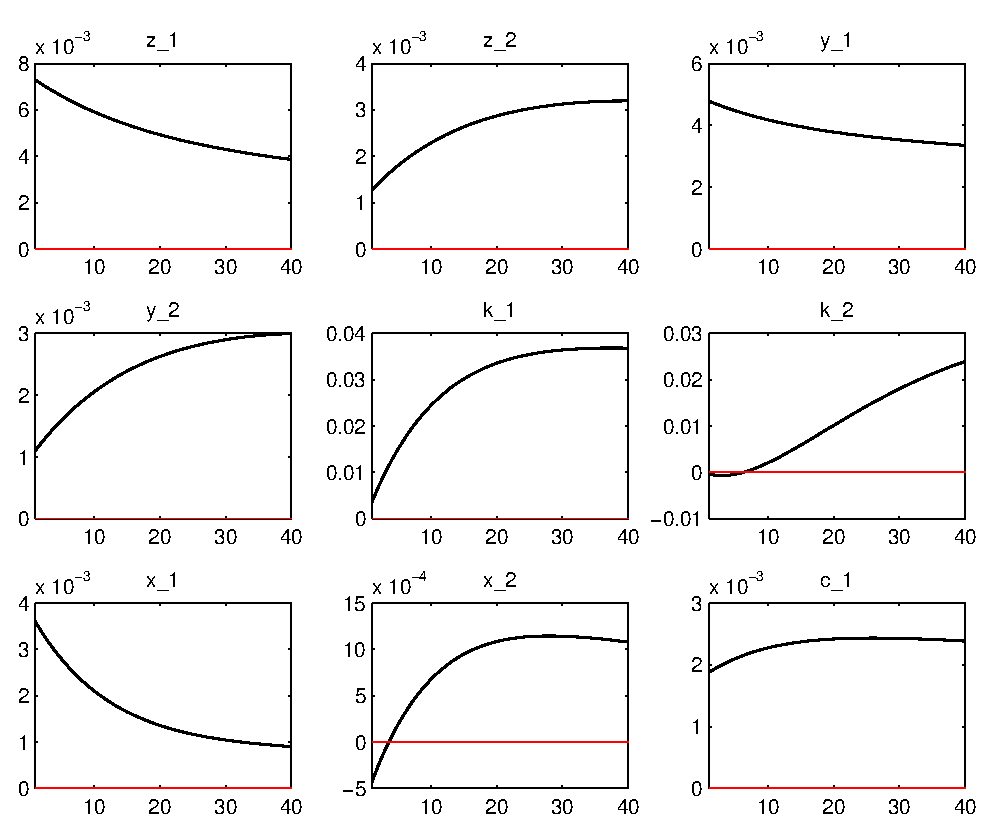
\includegraphics[scale=0.8]{dsge2_IRF_eps_11.eps} 
\label{gdp_filter}
\end{center}
\end{figure}

\begin{figure}[H]
\begin{center}
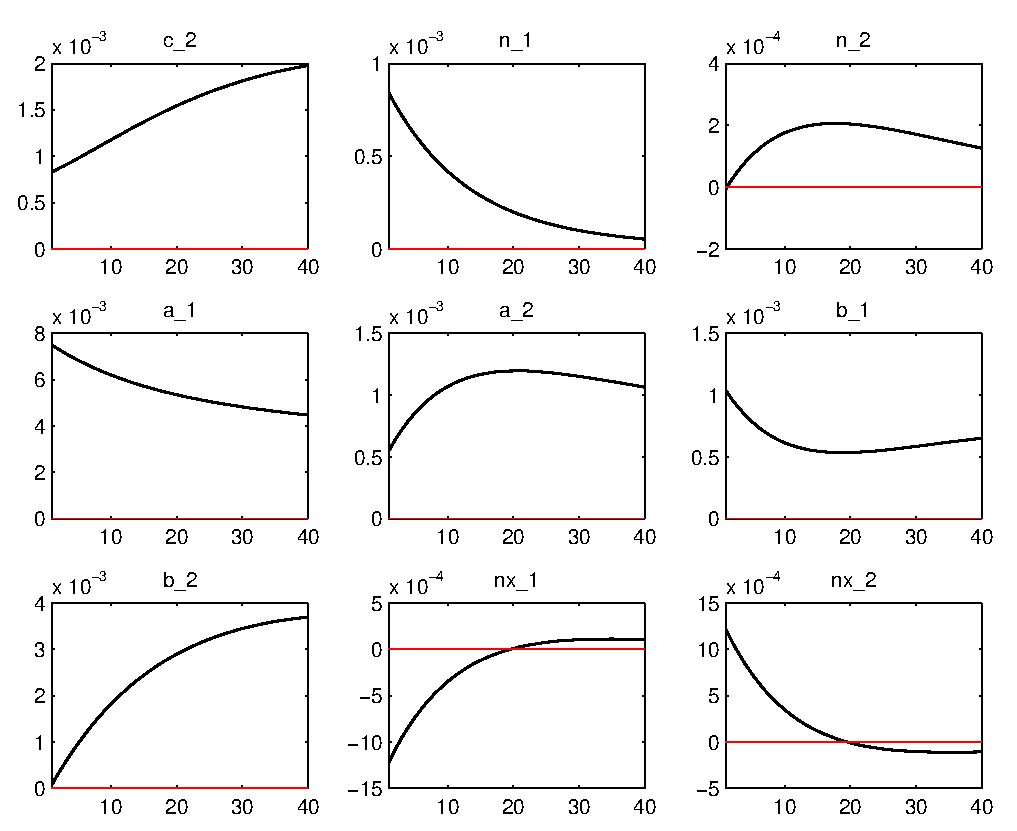
\includegraphics[scale=0.8]{dsge2_IRF_eps_12.eps} 
\label{gdp_filter}
\end{center}
\end{figure}
\begin{figure}[H]
\begin{center}
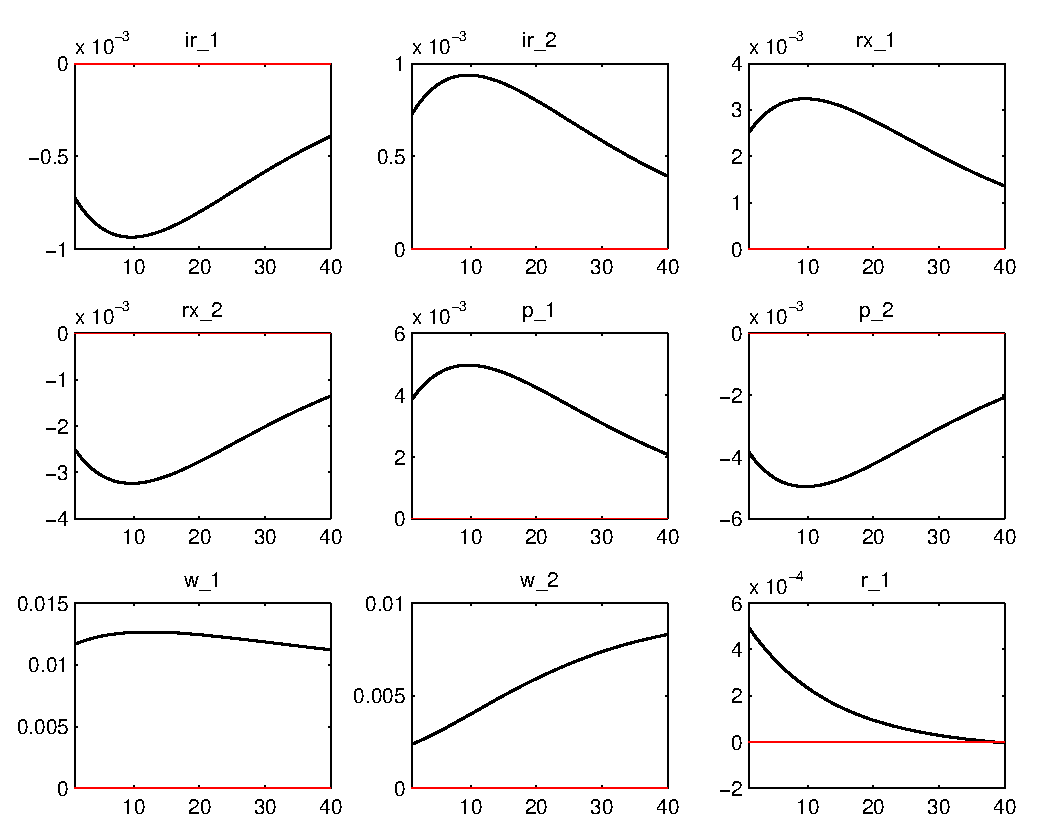
\includegraphics[scale=0.8]{dsge2_IRF_eps_13.eps} 
\label{gdp_filter}
\end{center}
\end{figure}

\subsection{Robustness Check: Home Bias}
\begin{table}[H]
\begin{center}
\begin{tabular}{ccccc}
\hline
\hline  
                                & $\omega=0.5$ & $\omega=0.75$ & $\omega=0.9$ &Benchmark\\
                                \hline
$corr(y_1,y_2)-corr(c_1,c_2)$    &              &               &            &  \\
Data                             &   0.22           &               &           &   \\
Complete market                  &   -0.01          &     -0.16          &    -0.36&   -0.30      \\
                                 &              &               &              &\\
$corr(x_1,x_2)$                    &              &               &             & \\
Data                             &    0.30          &               &            &  \\
Complete market                  &    0.16          &    -0.35           &    -0.30&   -0.33       \\
                                 &              &               &              &\\
\% std. dev. terms of trade (p) &              &               &              &\\
Data                             &    3.00          &               &          &    \\
Complete market                  &    1.00          &     0.81          &     0.62&    0.68     \\
\hline
\hline
\end{tabular}
\end{center}
\end{table}








\centering
\textbf{Appendix}
\appendix
\section{HP Filter: Python Code}
\lstset{language=Python,backgroundcolor=\color{white},numbers=left,basicstyle=\footnotesize,breaklines=true,frame=single}
\begin{lstlisting}
import os 
import numpy as np
import matplotlib.pylab as plt
import math

# HP filter of the data
# database is downloaded from perri's website

# set the working directory
os.chdir("/home/xuliheng/github/TestEcon/dsge")
os.getcwd()

# read csv data and convert it to ndarray
data_type="|S6,"+"<f8,"*10+"<f8"
data =np.genfromtxt('data.csv',dtype=data_type,delimiter=',',names=True)
print data.dtype.names
# GDP data
gdp = [math.log(i) for i in data["GDP"]]

# HP filter of GDP
import statsmodels.api as sm 
gdp_cycle, gdp_trend =sm.tsa.filters.hpfilter(gdp,1600)
'''
plt.plot(gdp,'-r')
plt.plot(gdp_trend,'-b')
plt.xlabel('period')
plt.ylabel('log(GDP)')
plt.show()
'''
# std of GDP
gdp_std = np.std(gdp_cycle)
print gdp_std 
# filter of other variables
var_std = {}
var_std["GDP"]= gdp_std
var_corr = {}
# filter of other variables
for i in range(2,12):
    var_name = data.dtype.names[i]
    if var_name != "Net_Exports":
        var = [math.log(j) for j in data[var_name]]
    else:
	var = data[var_name]
    #debug
    #if i==2:
    #    print var_name
    var_cycle,var_trend = sm.tsa.filters.hpfilter(var,1600)
    var_corr[var_name] = np.corrcoef(gdp_cycle,var_cycle)[0][1]
    if var_name in ["Total_C","GFCF","Civilian_Emp"]:
        var_std[var_name]=np.std(var_cycle)/gdp_std      
        #if i==2:
        #   print var_std 
    else:
        var_std[var_name]=np.std(var_cycle)
print var_std 
print var_corr

across_corr={}
data2_type="|S6,"+"<f8,"*3+"<f8"
data2 =np.genfromtxt('data2.csv',dtype=data2_type,delimiter=',',names=True)
for i in range(1,5):
    var_name = data2.dtype.names[i]
    var_2 = [math.log(k) for k in data2[var_name]]
    var_1 = [math.log(k) for k in data[var_name]]
    var_1_cycle,var_1_trend = sm.tsa.filters.hpfilter(var_1,1600)
    var_2_cycle,var_2_trend = sm.tsa.filters.hpfilter(var_2,1600)
    across_corr[var_name]=np.corrcoef(var_1_cycle,var_2_cycle)[0][1]
print across_corr
\end{lstlisting}




\section{The Full Dynare Code}
\lstset{language=Matlab,backgroundcolor=\color{white},numbers=left,basicstyle=\footnotesize,breaklines=true,frame=single}
\begin{lstlisting}
var z_1,z_2,y_1,y_2,k_1, k_2, x_1, x_2, c_1, c_2, n_1,n_2, a_1, a_2, b_1, b_2,nx_1,nx_2,ir_1,ir_2,rx_1,rx_2,p_1,p_2, w_1,w_2,r_1,r_2,qa_1,qa_2,qb_1,qb_2,lambda_1,lambda_2,f_1,f_2,yy_1,kk_1,xx_1,cc_1,aa_1,bb_1,nn_1,rr_1,yy_2,kk_2,xx_2,cc_2,aa_2,bb_2,nn_2,rr_2;
varexo eps_1, eps_2;

parameters beta, mu, gamma, theta, delta, rho, omega, A_1_1, A_1_2, A_2_1, A_2_2;

beta = 0.99;
mu   = 0.34;
gamma = -1;
theta =0.36;
delta = 0.025;
rho = -1/9;
omega = 0.85;
A_1_1=0.97;
A_1_2=0.025;
A_2_1=0.025;
A_2_2=0.97;

model;
//shock
z_1 = A_1_1 * z_1(-1) + A_1_2*z_2(-1)+eps_1;
z_2 = A_2_1 * z_1(-1) + A_2_2*z_2(-1)+eps_2;

//output
f_1=exp(z_1)*k_1(-1)^theta*n_1^(1-theta);
f_2=exp(z_2)*k_2(-1)^theta*n_2^(1-theta);

//feasibale constraint
x_1+c_1= (omega*a_1^rho+(1-omega)*b_1^rho)^(1/rho);
x_2+c_2= ((1-omega)*a_2^rho+omega*b_2^rho)^(1/rho);

// capital formation
k_1 = x_1+(1-delta)*k_1(-1);
k_2 = x_2+(1-delta)*k_2(-1);

// intermediate good
a_1+ a_2 = f_1;
b_1+ b_2 = f_2;

// wage in price of intermediate good
w_1 = (1-theta)*f_1/n_1;
w_2 = (1-theta)*f_2/n_2;

// Lagragian
lambda_1 = mu*((c_1^mu*(1-n_1)^(1-mu))^gamma)/c_1;
lambda_2 = mu*((c_2^mu*(1-n_2)^(1-mu))^gamma)/c_2;

// interest rate in price of intermediate good
r_1 =  theta*f_1/k_1(-1);
r_2 =  theta*f_2/k_2(-1);

// intermediate good pricing
qa_1 = omega*a_1^(rho-1)*((omega*a_1^rho+(1-omega)*b_1^rho)^(1/rho-1));
qb_1 = (1-omega)*b_1^(rho-1)* ((omega*a_1^rho+(1-omega)*b_1^rho)^(1/rho-1));
qa_2 = (1-omega)*a_2^(rho-1)*(((1-omega)*a_2^rho+omega*b_2^rho)^(1/rho-1));
qb_2 = omega*b_2^(rho-1)*(((1-omega)*a_2^rho+omega*b_2^rho)^(1/rho-1));

// foc to labor
(1-mu)*((c_1^mu*(1-n_1)^(1-mu))^gamma)/(1-n_1) = (lambda_1*qa_1)*w_1;
(1-mu)*((c_2^mu*(1-n_2)^(1-mu))^gamma)/(1-n_2) = (lambda_2*qb_2)*w_2;

//foc to capital
beta*lambda_1(1)*(qa_1(1) * r_1(1)+1-delta)=lambda_1;
beta*lambda_2(1)*(qb_2(1) * r_2(1)+1-delta)=lambda_2;

//foc to a_1
lambda_1* qa_1 =lambda_2* qa_2;

//foc to b_1
lambda_1* qb_1= lambda_2* qb_2;

// gdp    
y_1=qa_1*f_1;
y_2=qb_2*f_2;

//net export ratio
nx_1=(qa_1*a_2-qb_1*b_1)/y_1;
nx_2=(qb_2*b_1-qa_2*a_2)/y_2;

//import ratio
a_1*ir_1=b_1;
b_2*ir_2=a_2;

//terms of trade
qa_1*p_1=qb_1;
qb_2*p_2=qa_2;

//real exchange rate
rx_1*qa_2=qa_1;
rx_2*qa_1=qa_2;
kk_1=log(k_1);
nn_1 = log(n_1);
xx_1 =log(x_1);
cc_1=log(c_1);
aa_1=log(a_1);
bb_1=log(b_1);
rr_1 =log(r_1);
yy_1=log(y_1);
kk_2=log(k_2);
nn_2 = log(n_2);
xx_2 =log(x_2);
cc_2=log(c_2);
aa_2=log(a_2);
bb_2=log(b_2);
rr_2 =log(r_2);
yy_2=log(y_2);
end;

initval;
k_1=5.84336;
k_2=5.84336;
x_1=0.146084;
x_2=0.146084;
c_1=0.42366;
c_2=0.42366;
n_1=0.307182;
n_2=0.307182;
f_1=0.887017;
f_2=0.887017;
y_1=0.569744;
y_2=0.569744;
rx_1=1;
rx_2=1;
ir_1=0.209896;
ir_2=0.209896;
p_1=1;
p_2=1;
nx_1=1.39e-09;
nx_2=-3.30e-10;
eps_1=0;
eps_2=0;
z_1=0;
z_2=0;
a_1=0.733135;
a_2=0.153882;
b_1=0.153882;
b_2=0.733135;
w_1 =1.84806;
w_2 = 1.84806;
r_1 =  0.0546477;
r_2 =  0.0546477;
qa_1 = 0.642314;
qb_1 = 0.642314;
qa_2 = 0.642314;
qb_2 = 0.642314;
lambda_1 = 1.3692;
lambda_2 = 1.3692;
kk_1=log(k_1);
nn_1 = log(n_1);
xx_1 =log(x_1);
cc_1=log(c_1);
aa_1=log(a_1);
bb_1=log(b_1);
rr_1 =log(r_1);
yy_1=log(y_1);
kk_2=log(k_2);
nn_2 = log(n_2);
xx_2 =log(x_2);
cc_2=log(c_2);
aa_2=log(a_2);
bb_2=log(b_2);
rr_2 =log(r_2);
yy_2=log(y_2);
end;


steady;
check;

shocks;
var eps_1=0.0073^2;
var eps_2=0.0044^2;
var eps_1, eps_2= 0.29*0.0073*0.0044;
end;

stoch_simul(periods=2000,order=1,ar=10,hp_filter=1600,replic=1000,graph_format = eps);
\end{lstlisting}



\end{document}